\documentclass[12pt,a4paper]{report}
\usepackage[brazil]{babel}
\usepackage[]{algorithm}
\usepackage[]{algorithmic}

\usepackage[style=numeric,backend=biber]{biblatex}
\usepackage[utf8]{inputenc}
\usepackage{kpfonts}
\usepackage[T1]{fontenc}
\usepackage{wrapfig}
\usepackage{graphicx}
\usepackage{enumerate}
\usepackage{subcaption}
\usepackage{float}
\usepackage{caption}
\usepackage{listings}
\usepackage{lipsum}
\usepackage{amsthm}
\usepackage{amssymb}
\usepackage{bm}
\usepackage{color}
\usepackage{afterpage}
\usepackage[inline]{enumitem}
\usepackage{pdflscape}
\usepackage{listingsutf8}
\usepackage{siunitx}
\usepackage{bashful}

\usepackage[margin=1in]{geometry}

\lstset{frame=tb,
  aboveskip=2mm,
  belowskip=2mm,
  showstringspaces=false,
  columns=flexible,
  basicstyle=\footnotesize,,
  numbers=left,
  numbersep=5pt,
  stepnumber=1,
  breaklines=true,
  keepspaces=true,
  breakatwhitespace=true,
  showtabs=false,  
  tabsize=2
}


% Definindo estilo para os códigos
\definecolor{mGreen}{rgb}{0,0.6,0}
\definecolor{mGray}{rgb}{0.5,0.5,0.5}
\definecolor{mPurple}{rgb}{0.58,0,0.82}
\definecolor{dkgreen}{rgb}{0,0.6,0}
\definecolor{backgroundColour}{rgb}{0.97,0.97,0.97}

\lstset{basicstyle=\ttfamily,
    backgroundcolor=\color{backgroundColour},   
    commentstyle=\color{mGreen},
    keywordstyle=\color{magenta},
    numberstyle=\tiny\color{mGray},
    commentstyle=\color{dkgreen},
    stringstyle=\color{mPurple},
    basicstyle=\footnotesize,
    breakatwhitespace=false\textbf{,}         
    breaklines=true,                 
    captionpos=b,                    
    keepspaces=true,                 
    numbers=left,                    
    numbersep=5pt,                  
    showspaces=false,                
    showstringspaces=false,
    showtabs=false,                  
    tabsize=2,
    language=bash
}

\lstdefinestyle{BStyle}{
    backgroundcolor=\color{backgroundColour},  
    showstringspaces=false,
    numbers=none,
    language=bash
}

\pagenumbering{arabic}
\renewcommand{\thesection}{\arabic{section}}

\bibliography{ref}
\renewcommand{\contentsname}{Sumário}{\thispagestyle{empty}}
\renewcommand{\baselinestretch}{1.5} 

\begin{document}

\begin{titlepage}
        \begin{center}
                \vspace*{1cm}
                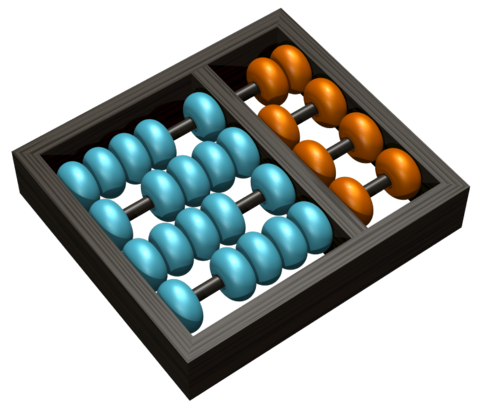
\includegraphics[width=0.25\textwidth]{Logo}\\
                \vspace{1.5cm}
                \Huge
                \textbf{Exercício 2}\\
                \vspace{1.5cm}
                \Large
                \textbf{Aluno}: João Vitor Gonçalves\\
                \textbf{RA}: 176353\\
                \vspace{1.2cm}
                \Large
                Instituto de Computação\\
                Universidade Estadual de Campinas\\
                \vspace{1.5cm}
                Campinas, 18 de Outubro de 2020.
        \end{center}
\end{titlepage}
\tableofcontents
\clearpage

\newcommand{\shellcmd}[1]{\texttt{\footnotesize\# #1}}%estilizando citação de comandos do shell

% \section{Insertion Sort}

% \subsubsection{Pseudocódigo}
% \begin{algorithm}
% \caption{InsertionSort(A)}
% \begin{algorithmic}[1]
%     \STATE $A[0] \longleftarrow -\alpha$
%   \STATE $i \longleftarrow 2 $
%     \FOR {$i$ to $N $} 
%             \STATE $j \longleftarrow i$

%             \WHILE{$A[j] > A[j-1]$} 
%                 \STATE $T \longleftarrow A[j-1]$ 
%                 \STATE $A[j-1] \longleftarrow A[j]$ 
%                 \STATE $A[j] \longleftarrow T$ 
%                 \STATE $j = j -1$
%             \ENDWHILE
%     \ENDFOR
%     \RETURN $A$
%     \end{algorithmic}
% \end{algorithm}



\section{ifconfig}

\subsection{Qual opção deve ser usada para exibir informações sobre todas as interfaces de rede?}

O comando \emph{ifconfig} quando executado sem argumentos, lista as interfaces de rede ativas. eg:

\begin{lstlisting}[language=bash]
$ ifconfig
\end{lstlisting}

\noindent Para mostrar todas as interfaces de rede, ele deve ser executado com a flag \textbf{-a}

\begin{lstlisting}[language=bash]
$ ifconfig -a
br-a10973c7ec6c: flags=4099<UP,BROADCAST,MULTICAST>  mtu 1500
        inet 172.19.0.1  netmask 255.255.0.0  broadcast 172.19.255.255
        ether 02:42:b8:fe:ac:23  txqueuelen 0  (Ethernet)
        RX packets 0  bytes 0 (0.0 B)
        RX errors 0  dropped 0  overruns 0  frame 0
        TX packets 0  bytes 0 (0.0 B)
        TX errors 0  dropped 0 overruns 0  carrier 0  collisions 0

docker0: flags=4099<UP,BROADCAST,MULTICAST>  mtu 1500
        inet 172.17.0.1  netmask 255.255.0.0  broadcast 172.17.255.255
        ether 02:42:2b:e6:81:df  txqueuelen 0  (Ethernet)
        RX packets 0  bytes 0 (0.0 B)
        RX errors 0  dropped 0  overruns 0  frame 0
        TX packets 0  bytes 0 (0.0 B)
        TX errors 0  dropped 0 overruns 0  carrier 0  collisions 0

eno1: flags=4163<UP,BROADCAST,RUNNING,MULTICAST>  mtu 1500
        inet 192.168.100.128  netmask 255.255.255.0  broadcast 192.168.100.255
        inet6 fe80::6799:e59a:3a29:3c46  prefixlen 64  scopeid 0x20<link>
        ether 00:d8:61:6f:ea:50  txqueuelen 1000  (Ethernet)
        RX packets 5253629  bytes 6151206386 (6.1 GB)
        RX errors 0  dropped 0  overruns 0  frame 0
        TX packets 1812540  bytes 191417863 (191.4 MB)
        TX errors 0  dropped 0 overruns 0  carrier 0  collisions 0
        device interrupt 16  memory 0xa4200000-a4220000  

lo: flags=73<UP,LOOPBACK,RUNNING>  mtu 65536
        inet 127.0.0.1  netmask 255.0.0.0
        inet6 ::1  prefixlen 128  scopeid 0x10<host>
        loop  txqueuelen 1000  (Local Loopback)
        RX packets 808745  bytes 648198978 (648.1 MB)
        RX errors 0  dropped 0  overruns 0  frame 0
        TX packets 808745  bytes 648198978 (648.1 MB)
        TX errors 0  dropped 0 overruns 0  carrier 0  collisions 0    
\end{lstlisting}

\noindent Assim serão exibidas todas as interfaces, mesmo as desativadas.

\subsection{O que deve ser feito para exibir somente informações de uma interface específica?}

Para exibir informações de somente uma interface específica, o seu nome deve ser passado como um argumento para o comando:

\begin{lstlisting}[language=bash]
$ ifconfig br-a10973c7ec6c
br-a10973c7ec6c: flags=4099<UP,BROADCAST,MULTICAST>  mtu 1500
        inet 172.19.0.1  netmask 255.255.0.0  broadcast 172.19.255.255
        ether 02:42:b8:fe:ac:23  txqueuelen 0  (Ethernet)
        RX packets 0  bytes 0 (0.0 B)
        RX errors 0  dropped 0  overruns 0  frame 0
        TX packets 0  bytes 0 (0.0 B)
        TX errors 0  dropped 0 overruns 0  carrier 0  collisions 0
\end{lstlisting}

\section{nslookup}
\subsection{Quais são os endereços IP do host www.unicamp.br?}

\begin{lstlisting}[language=bash]
        $ nslookup www.unicamp.br
        Server:		127.0.0.53
        Address:	127.0.0.53#53

        Non-authoritative answer:
        www.unicamp.br	canonical name = 143-106-143-186.nuvem.unicamp.br.
        Name:	143-106-143-186.nuvem.unicamp.br
        Address: 143.106.143.186
\end{lstlisting}

O endereço retornado pelo \emph{nslookup} para o host \textbf{www.unicamp.br} é \emph{143.106.143.186}

\subsection{Há alguma vantagem em haver mais de um endereço IP?}

Existem sim algumas vantagens em se ter mais de um endereço IP para um domínio.

A primeira e mais óbvia é por questões de redundância. Caso o servidor que responde por um dos endereços se torne irresponsivo, existem endereços de outros servidores que ainda podem estar funcionando mantendo assim o serviço ativo, mesmo que parcialmente.

Outro motivo é por questões geograficas, onde podemos ter endereços IPs que apontem para sevidores mais próximos geograficamente dos usuários, diminuindo assim a latência de resposta.

Um terceiro motivo pode ser por questões de balanceamento de tráfego, caso exista mais de um endereço IP disponível para um domínio, as requisições serão direcionas de forma randômica entre eles, dividindo assim a carga total.

Existem inúmeros outros motivos pelos quais ter mais de um endereço IP pode ser desejável, mas resumindo, existem sim vantagens.

\section{traceroute}
\subsection{Quantos roteadores estão entre a sua estação e o host www.amazon.com? Pelos nomes dos roteadores, quantos deles estão localizados no Brasil?}

Executando o comando \emph{traceroute} para o endereço \emph{www.amazon.com} obtemos:

\begin{lstlisting}[language=bash]
        $ traceroute www.amazon.com   
        traceroute to www.amazon.com (13.33.130.223), 30 hops max, 60 byte packets
         1  _gateway (192.168.100.1)  0.390 ms  0.344 ms  0.288 ms
         2  192.168.0.1 (192.168.0.1)  1.439 ms  1.494 ms  1.341 ms
         3  10.21.0.1 (10.21.0.1)  14.750 ms  8.691 ms  14.799 ms
         4  c94c1001.virtua.com.br (201.76.16.1)  17.870 ms  17.867 ms  18.191 ms
         5  embratel-G0-5-3-2-tacc01.cas.embratel.net.br (200.174.243.53)  20.587 ms embratel-T0-3-0-0-uacc02.cas.embratel.net.br (189.16.179.53)  22.126 ms  22.086 ms
         6  ebt-H0-7-0-3-tcore01.cas.embratel.net.br (200.244.213.103)  33.239 ms ebt-H0-4-0-0-tcore01.cas.embratel.net.br (200.244.212.61)  36.143 ms ebt-H0-7-0-3-tcore01.cas.embratel.net.br (200.244.213.103)  24.095 ms
         7  ebt-B1191-tcore01.spo.embratel.net.br (200.230.252.130)  35.167 ms  33.017 ms  24.929 ms
         8  ebt-B2111-tcore01.rjo.embratel.net.br (200.230.251.1)  37.181 ms  31.957 ms  33.497 ms
         9  ebt-H0-2-0-1-uacc04.rjoen.embratel.net.br (200.244.211.210)  30.454 ms  30.465 ms ebt-H0-7-0-1-uacc04.rjoen.embratel.net.br (200.244.211.214)  30.384 ms
        10  peer-B55-uacc04.rjoen.embratel.net.br (189.87.140.110)  30.038 ms  28.433 ms  28.439 ms
        11  52.93.67.58 (52.93.67.58)  27.497 ms peer-B55-uacc04.rjoen.embratel.net.br (189.87.140.110)  26.865 ms  21.708 ms
        12  52.93.67.197 (52.93.67.197)  30.382 ms 52.93.67.199 (52.93.67.199)  30.470 ms *
        13  * * *
        ...
\end{lstlisting}

Cosiderando o roteador \emph{gateway} local, temos um total de 12 roteadores entre a minha interface de rede e o host \emph{www.amazon.com}.

Podemos observar que até o roteador de número \textbf{10}, os roteadores estão localizados no Brasil, uma vez que possuem nomes relacionados à Embratel ou à Net Virtua.
E a partir do roteador \textbf{11}, podemos observar por meio do comando \emph{whois} que os endereços dos roteadores \emph{11} e \emph{12} são pertencentes à \emph{amazon}.

\begin{lstlisting}[language=bash]
        $whois 52.93.67.58
        ... 
        OrgName:        Amazon Technologies Inc.
        OrgId:          AT-88-Z
        Address:        410 Terry Ave N.
        City:           Seattle
        StateProv:      WA
        PostalCode:     98109
        Country:        US
        ...
\end{lstlisting}


\begin{lstlisting}[language=bash]
        $whois 52.93.67.197
        ... 
        OrgName:        Amazon Technologies Inc.
        OrgId:          AT-88-Z
        Address:        410 Terry Ave N.
        City:           Seattle
        StateProv:      WA
        PostalCode:     98109
        Country:        US
        ...
\end{lstlisting}





\section{telnet}
\subsection{É possível conectar-se com este comando em um servidor HTTP? Se sim, como deve-se executar o comando para conectar-se no host www.amazon.com na porta padrão do HTTP?}
É possível sim conectar-se a um servidor \textbf{HTTP} utilizando o \emph{telnet}, para isso é necessário especificar qual porta à ser utilizada, que no caso do \textbf{HTTP} é por padrão a porta \textbf{80}.
\begin{lstlisting}[language=bash]
        $ telnet amazon.com 80
        Trying 176.32.103.205...
        Connected to amazon.com.
        Escape character is '^]'.
\end{lstlisting}


\subsection{Caso não haja um servidor escutando na porta passada pelo comando telnet, o que ocorre? Justifique.}

Caso não exista um servidor na porta passada para o \emph{telnet} a conexão não é estabelecida, uma vez que é necessário existir um processo sendo executado na porta requisitada para que seja possível estabelecer uma conexão \emph{TCP} para o telnet criar um terminal remoto e enviar comandos.
\begin{lstlisting}[language=bash]
        $ telnet amazon.com 81
        Trying 176.32.98.166...
        Trying 176.32.103.205...
        Trying 205.251.242.103...
        telnet: Unable to connect to remote host: Connection refused
\end{lstlisting}



\subsection{A qual a camada da rede o telnet pertence?}
O telnet pertence à camada de \textbf{Aplicação}, uma vez que ele é um protocolo criado para enviar comandos de outros procolos de \textbf{Aplicação} como HTTP e FTP, por meio do protocolo da camada de transporte \textbf{TCP}.


\section{Acesse o site da DAC (https://www.dac.unicamp.br/) e, em paralelo em um terminal, verifique a saída do comando netstat. Quais são as informações fornecidas a respeito da conexão ao site da DAC?}
Iremos utilizar o comando \emph{netstat} em conjunto com as flags \emph{-antp}, onde:
\begin{itemize}
        \item \textbf{-a}: Mostra todos os sockets, estabelecidos (\emph{listening} e \emph{non-listening} no caso do TCP).
        \item \textbf{-n}: Exibe os valores numéricos dos endereços, sem realizar uma resolução.
        \item \textbf{-t}: Exibe somente as conexões \emph{TCP} estabelecidas.
        \item \textbf{-p}: Exibe o \emph{PID} do processo a qual o socket pertence, que no caso serão \emph{PIDs} do Chrome para a conexão ao site da DAC.
\end{itemize}

Então executando o comando, com o site da DAC aberto obtemos:

\begin{lstlisting}[language=bash]
        $ netstat -antp   
        (Not all processes could be identified, non-owned process info
         will not be shown, you would have to be root to see it all.)
        Active Internet connections (servers and established)
        Proto Recv-Q Send-Q Local Address           Foreign Address         State       PID/Program name    
        ...
        tcp        0      0 192.168.100.128:45824   143.106.227.165:443     ESTABLISHED 25502/chrome --type 
        ...
\end{lstlisting}

Onde é possível observar a conexão TCP entre o servidor do site da DAC e o host local.

Então nesse caso temos uma conexão do hospedeiro local na porta \emph{45824} para o servidor da DAC (\emph{143.106.227.165}) na porta \emph{443}.

Além disso temos o estado da conexão \textbf{HTTP} que no caso é \emph{ESTABLISHED} e o PID do processo local que é dono desse socket, que no caso é o Chrome com PID \emph{25502}.

Além dessa conexão por onde foi transmitido o documento da página em si, foram abertas outras conexões para a obtenção de recursos requisitados pelo documento \textbf{HTML}, como por exemplo fontes de texto requisitadas para o servidor da Google, que gerou a seguinte conexão:

\begin{lstlisting}[language=bash]
        $ netstat -antp   
        ...
        tcp        0      0 192.168.100.128:51450   172.217.173.74:443      ESTABLISHED 25502/chrome --type 
        ...
\end{lstlisting}

Filtrando os resultados do \emph{netstat} para todas as conexões contendo o endereço IP da DAC, temos:

\begin{lstlisting}[language=bash]
        $ netstat -antp | grep "143.106.227.165:443"  
        (Not all processes could be identified, non-owned process info
        will not be shown, you would have to be root to see it all.)
        tcp        0      0 192.168.100.128:43234   143.106.227.165:443     ESTABLISHED 5429/chrome --type= 
        tcp        0      0 192.168.100.128:43232   143.106.227.165:443     ESTABLISHED 5429/chrome --type= 
        tcp        0      0 192.168.100.128:43244   143.106.227.165:443     ESTABLISHED 5429/chrome --type= 
\end{lstlisting}

Ou seja, foram criadas 3 conexões TCP entre o hospedeiro local e o servidor da DAC ao acessar o site. Isso pode ser feito pelo navegador como forma de carregar objetos da página HTML de forma concorrente.

\section{TCPDUMP}
\subsection{Utilizando o TCPDUMP corretamente com os filtros é possível somente capturar o tráfego HTTPS? Se sim, execute o comando junto com os filtros e anexe uma figura que comprove sua resposta no relatório. Se sua resposta foi não, então justifique-a.}

É possível sim, podemos capturar o tráfego HTTPS por meio do comando \emph{tcpdump -nnSX port 443}, onde o mais importante no comando é o filtro pela porta \textbf{443}, que é por onde é feito a transferência dos pacotes criptografados do \emph{HTTPS}.

As flags passadas \emph{nnSX} são utilizadas para mostrar o conteúdo de cada pacote interceptado (-X) e formatar a saída, como não converter endereços IP (-n) e mostrar o valor absoluto do número de sequência dos pacotes TCP (-S).

\begin{figure}[H]
        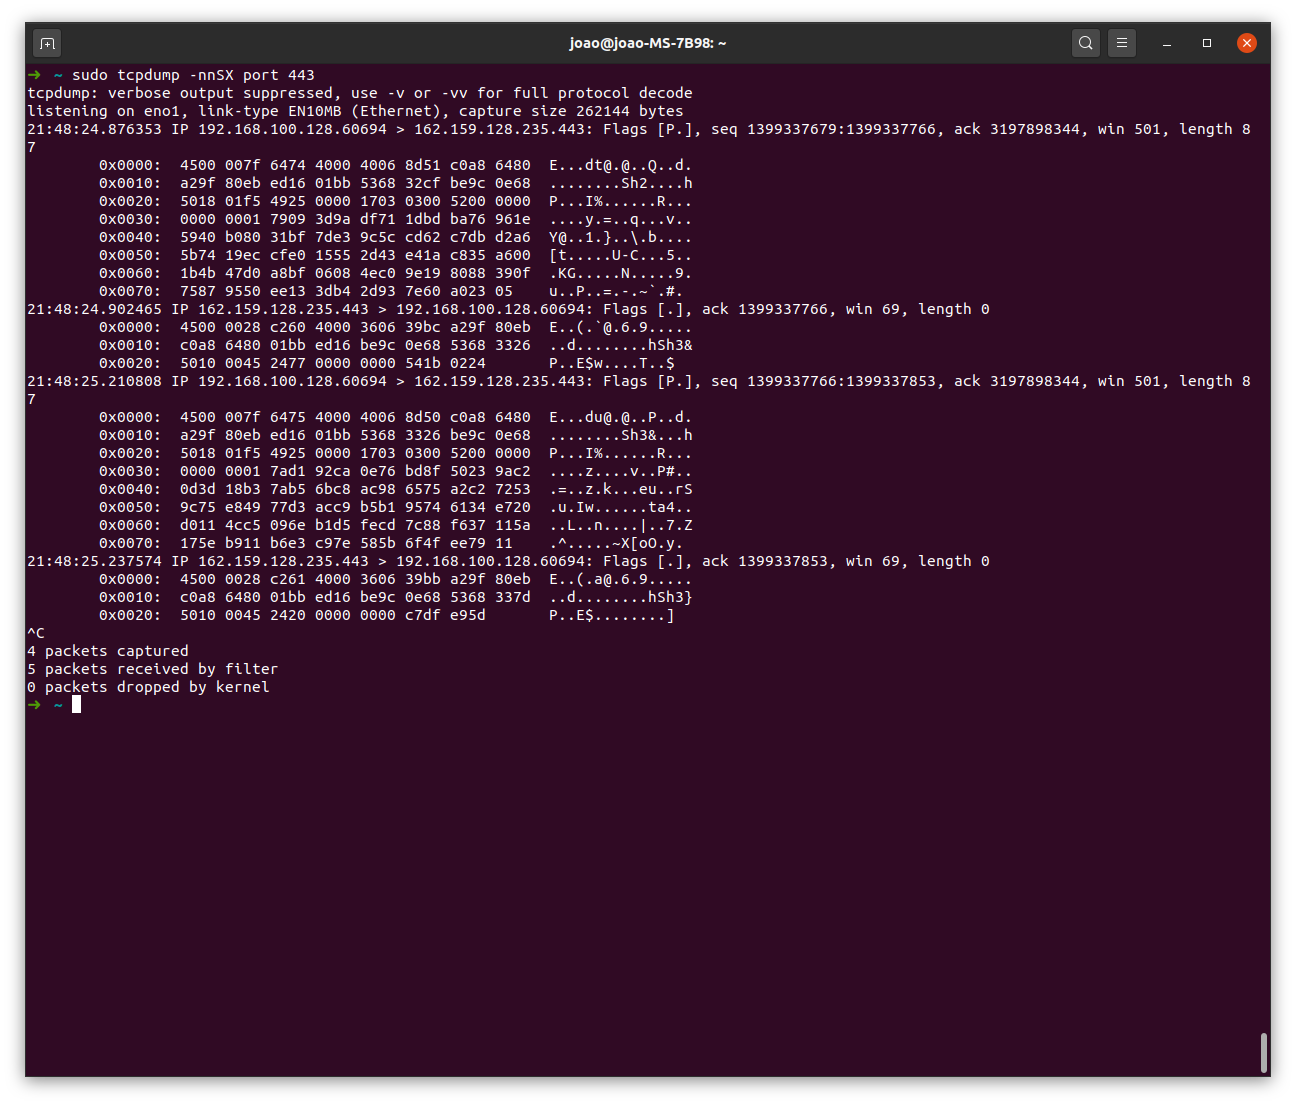
\includegraphics[width=\linewidth]{tcpdump.png}
        \caption{Execução do comando tcpdump para capturar pacotes HTTPS.}
\end{figure}

\subsection{Utilizando o comando TCPDUMP seguido dos parâmetros corretos imprima somente os pacotes superiores a 64 bits. Indique qual foi a sequência de comandos utilizada.}

Por meio da execução do comando \emph{sudo tcpdump -nnSX port 443 and greater 8} é possível filtrar os pacotes pelos seus tamanhos. Em específico o filtro \emph{greater} que filtra os pacotes exibidos pelo seu tamanho em \emph{bytes}, ou seja, passando o valor \textbf{8} selecionamos apenas pacotes com tamanho maior que 64 bits.

\begin{figure}[H]
        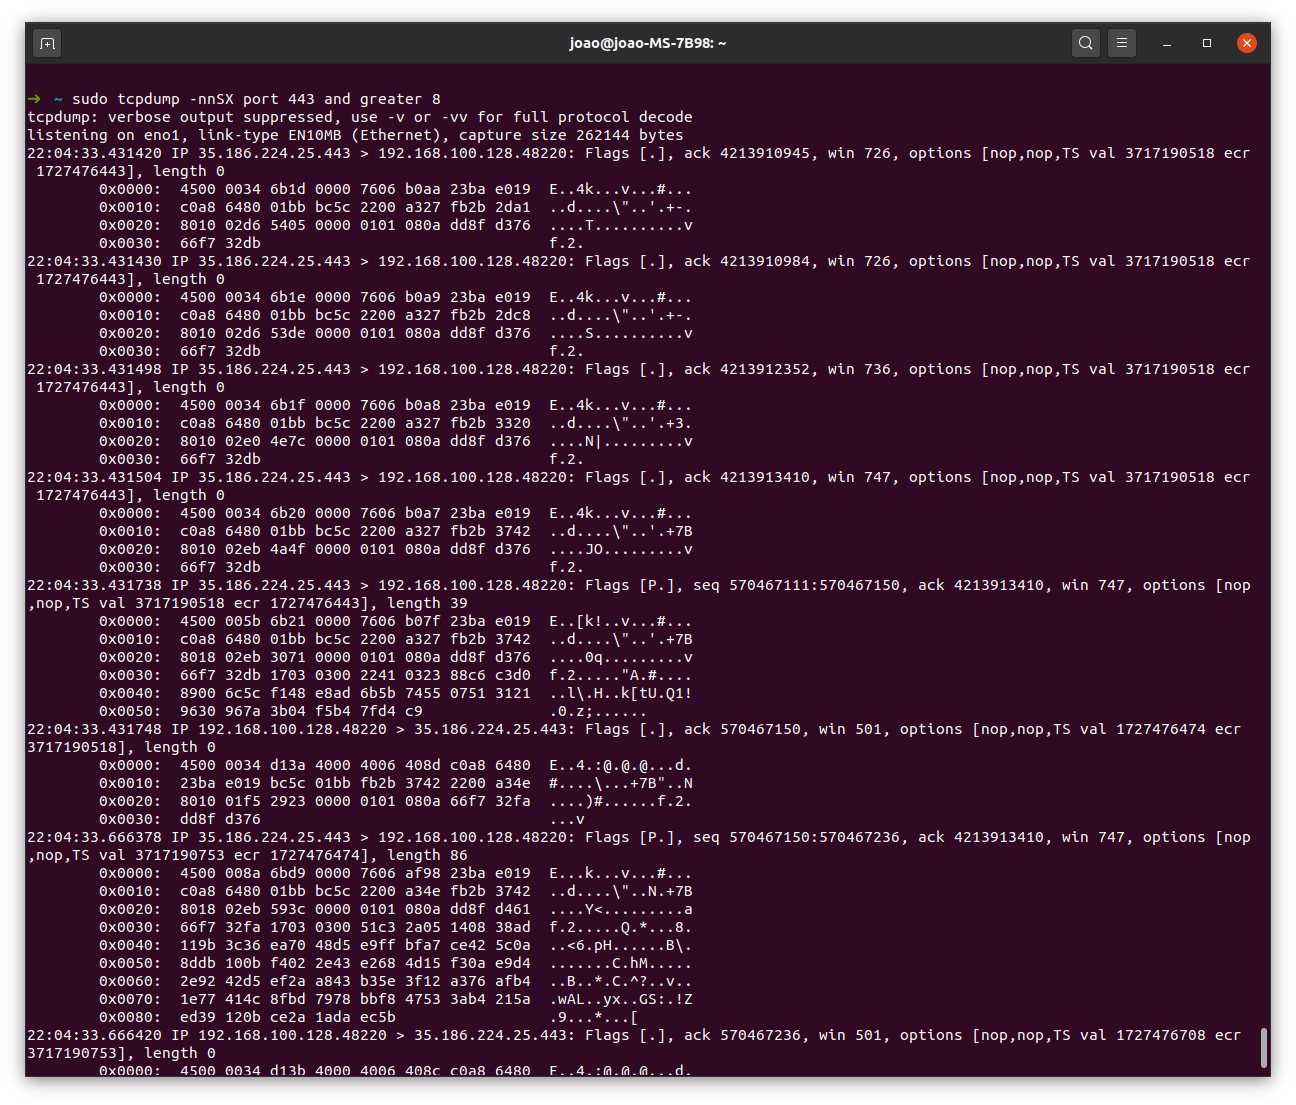
\includegraphics[width=\linewidth]{tcpdump64.png}
        \caption{Execução do comando tcpdump para capturar pacotes HTTPS maiores que 64 bits (8 bytes).}
\end{figure}


\subsection{Utilizando o TCPDUMP seguido de filtros, imprima somente os resultados que tiverem a flag ‘ACK’. Insira o comando seguido dos filtros e uma figura no seu relatório para comprovar o sucesso.}

Podemos filtrar somente pacotes com flag \emph{ACK} por meio do comando:

\begin{lstlisting}[language=bash]
sudo tcpdump -nnSX "tcp[tcpflags] & (tcp-ack) != 0"
\end{lstlisting}


\begin{figure}[H]
        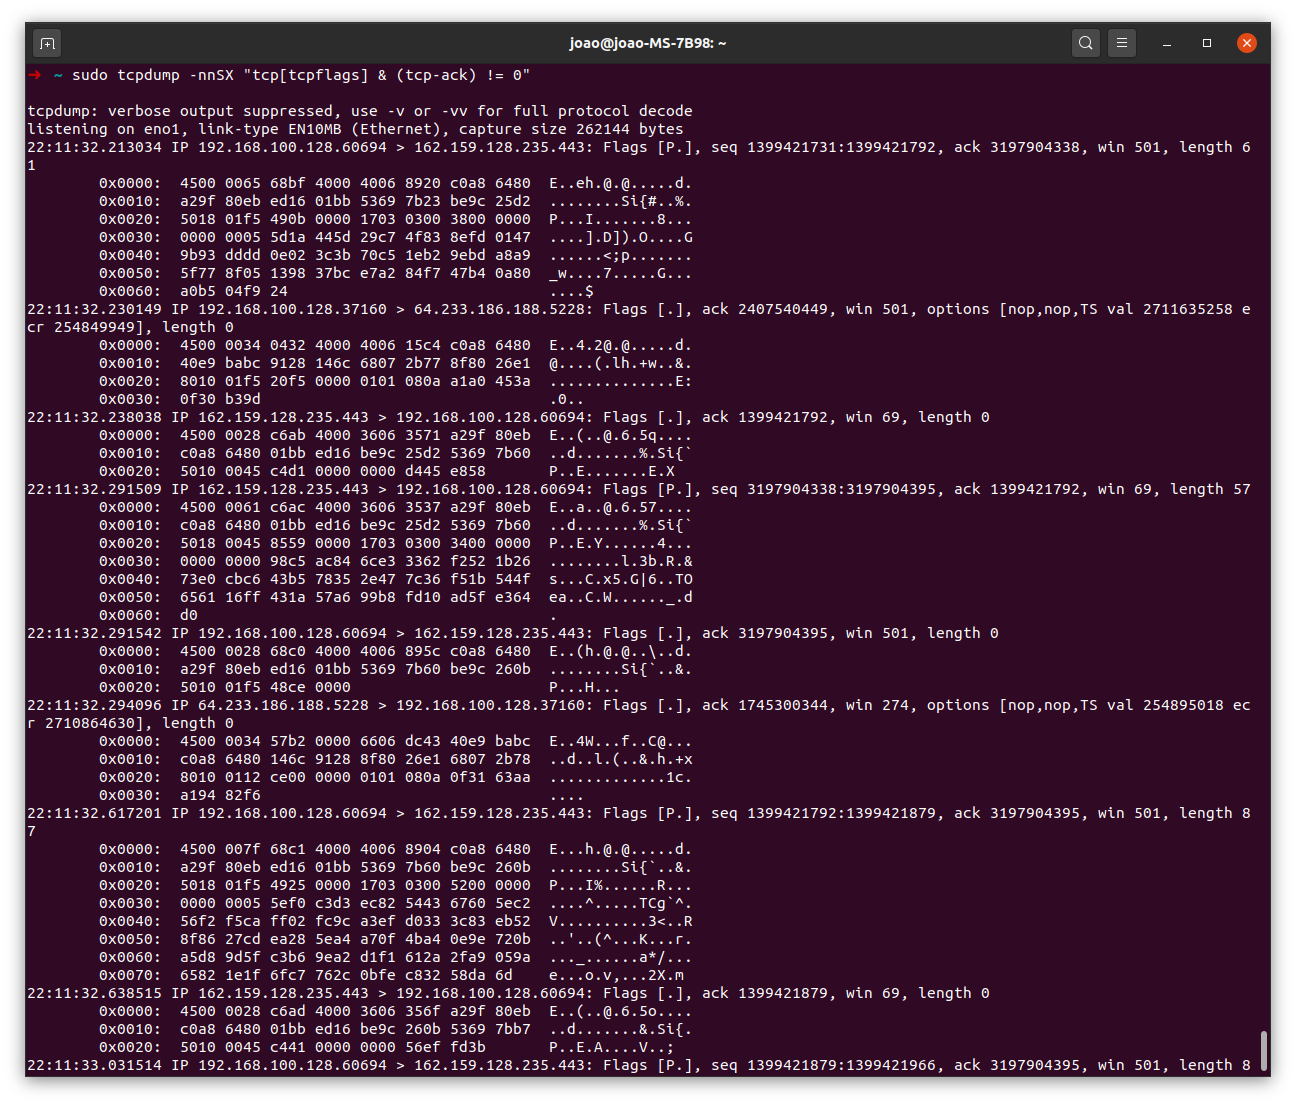
\includegraphics[width=\linewidth]{tcpdumpack.png}
        \caption{Execução do comando tcpdump para capturar pacotes com flag ACK.}
\end{figure}

\section{Wireshark}


\subsection{Comparado às demais ferramentas apresentadas na aula de MC833 descreva quais são principais diferenças e vantagens de usar o Wireshark? Escolha pelo menos uma ferramenta/sniffer e elabore uma tabela comparativa para responder a questão.}

Comparando o \emph{Wireshark} ao sniffer \emph{TCPDUMP}.
% https://www.youtube.com/watch?v=76BdFaJs_ts


\begin{table}[H]
        \begin{tabular}{|l|l|lll}
                \cline{1-3}
                                                & TCPDUMP & \multicolumn{1}{l|}{Wireshark} &  & \\ \cline{1-3}
                UI                              & CLI     & \multicolumn{1}{l|}{GUI}       &  & \\ \cline{1-3}
                API                             & libcap  & \multicolumn{1}{l|}{libcap}    &  & \\ \cline{1-3}
                Simple \emph{SSH} Remote Access & YES     & \multicolumn{1}{l|}{NO}        &  & \\ \cline{1-3}
                Isolate TCP Session Streams     & NO      & \multicolumn{1}{l|}{YES}       &  & \\ \cline{1-3}
        \end{tabular}
\end{table}

O Wireshark é um dos sniffers de rede mais conhecidos, tanto por ser extremamente versátil e de fácil utilização. Pelo fato de ele ser uma aplicação com interface gráfica, é mais simples de se obter informações necessárias sobre pacotes e acompanhar transmissões de uma certa conexão.
Comparativamente com o TCPDUMP, essa manipulação deve ser toda feita por seus filtros na linha de comando e manipulação do seu output com outras ferramentas de linha de comando como o \emph{awk} e o \emph{grep}.

Porém tecnicamente, como ambas as ferramentas utilizam a mesma api para realizar o monitoramento da rede, é possível fazer as mesmas análises com ambas, mesmo que sendo necessário o uso de ferramentas externas no caso do TCPDUMP.

Onde o TCPDUMP também leva uma certa vantagem é por ser uma ferramenta de linha de comando, uma vez que não é sempre possível de se utilizar uma interface gráfica, como em acessos à servidores remotos.

\subsection{Em uma rede com vários processos acontecendo ao mesmo tempo é possível gerenciar de forma isolada um único processo
        específico na rede utilizando ferramentas/sniffers apresentados nesta disciplina? Se sim, quais ferramentas e/ou sniffers você usaria?
        Justifique sua resposta. (OBS: Não é necessário apresentar comandos ou prints)}

É possível sim, e de forma realtivamente simples. Com ambos o TCPDUMP quanto o Wireshark, isso pode ser feito.
No caso do TCPDUMP isso é mais complexo, uma vez que não é possível filtrar as transmissões por um PID do processo.
Precisamos primeiro identificar ou o endereço que o processo está se comunicando, ou por quais portas por meio do \emph{netstat}.
Uma vez que isso é identificado, podemos simplesmente utilizar o filtro do TCPDUMP para mostrar somente pacotes que tenham essas
características.

Já o Wireshark oferece filtros que tornam essa tarefa mais simples. Com ele podemos simplesmente filtrar pacotes pelo nome do processo local (eg. \emph{chrome}).
Além disso com o Wireshark, é possível acompanhar as transferências de uma conexão TCP mais fácilmente, então uma vez identificada que conexão queremos monitorar, basta apenas filtrá-la.
\end{document}